\chapter{Reconstruction and Regression with Binary-Valued Graph Signals} % Main chapter title

\label{chap:binary} 

\lhead{Chapter 7. \emph{Reconstruction and Regression with Binary-Valued Graph Signals}} 

So far in this thesis, we have focused on reconstruction and regression models for real-valued graph signals, as discussed in \cref{chap:gsr_2d,chap:kgr_rnc_2d,chap:nd_gsp,chap:variance}. In this chapter, we shift our attention to scenarios where the signal of interest is binary-valued. Such signals can be employed to describe node classification tasks conducted over networks. For instance, consider the task of predicting whether users in a social network will click on a specific online advertisement. It is reasonable to assume that closely connected individuals within the network are more likely to have a similar probability of clicking than distantly connected individuals. Consequently, integrating this relational information into a predictive task may enhance accuracy. In this example, the classification task is binary as visualised in \cref{fig:binary_class_graph}. However, there may also be situations in which each node must be classified into one of many groups. In this case, we have a multiclass classification, as visualised in \cref{fig:mutliclass_graph}. \cite{Li2012}


\begin{figure}[t] 
    \begin{center}
        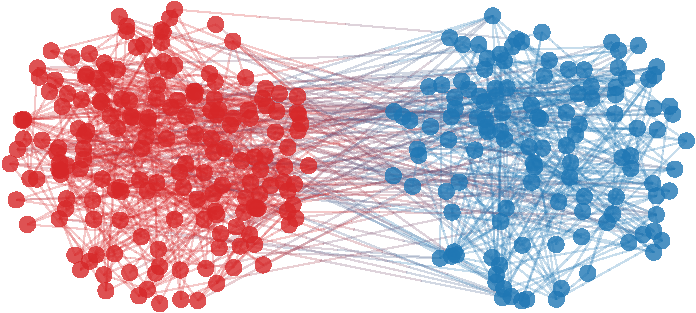
\includegraphics[width=0.8\linewidth]{Figures/2class_graph.pdf}
    \end{center}
   \caption[Visualisation of a binary classification task over a network]{An example visualisation of a binary classification task over a network.} 
    \label{fig:binary_class_graph}
\end{figure} 

\begin{figure}[t] 
    \begin{center}
        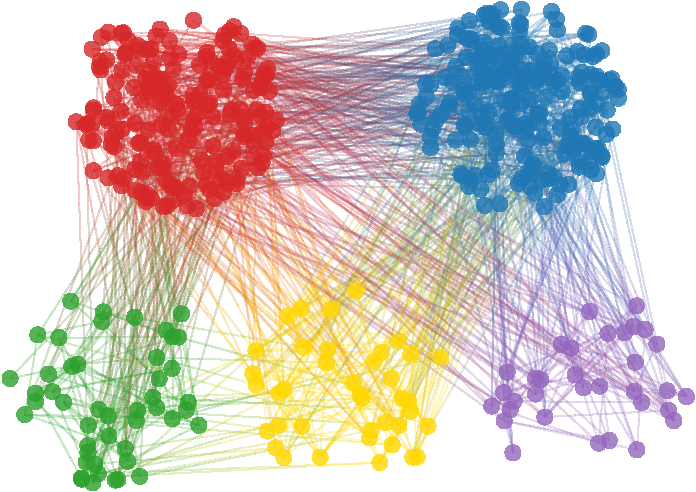
\includegraphics[width=0.8\linewidth]{Figures/multiclass_graph.pdf}
    \end{center}
   \caption[Visualisation of a multiclass classification task over a network]{An example visualisation of a multiclass classification task over a network.} 
    \label{fig:mutliclass_graph}
\end{figure} 



\section{Logistic Graph Signal Reconstruction}

\label{sec:lgsr}



Consider a binary signal reconstruction problem over a Cartesian product graph of order $d$. The observed graph signal, $\Yt$, is an order-$d$ tensor of shape $(N_1, N_2, .., N_d)$, with binary-valued elements. This is accompanied by another binary tensor, $\St$, of the same shape. As in previous chapters, $\St$ contains the information about which elements of $\Yt$ were observed by holding ones at elements where successful observations were made and zeros elsewhere. The goal is to predict the value of the graph signal at elements where no observation was made. 

\begin{equation*}
    \text{input data} = \Big\{\; \Yt \in \{0, 1\}^{N_1 \times ... \times N_d}, \;\; \St \in \{0, 1\}^{N_1 \times ... \times N_d} , \;\; \A \in \R^{N \times N} \; \Big\}
\end{equation*}

In the following, we assume each observed element, $\nn$, of the tensor, $\Yt$, follows a Bernoulli distribution with a mean $\Mt_\nn$. All other elements of $\Yt$ not in the set of observed elements $\mathcal{S}$ are zero with probability one. 

\begin{equation}
    \Yt_\nn \sim  \begin{cases}
        \text{Bern}\left(\Mt_\nn \right) & \text{if} \;\; \nn \in \mathcal{S} \\
        \text{Bern}\left(0\right) & \text{otherwise}
    \end{cases}
\end{equation}


$\Mt$ is the mean tensor, which has the same shape as $\Yt$ and elements falling within the interval $[0, 1]$. For a given mean, $\Mt$, the probability of observing a binary signal $\Yt$ is therefore given by 

\begin{equation}
    p(\Yt \, | \, \Mt) = \prod_{\nn \in \mathcal{S}} \Mt_\nn^{\Yt_\nn}\left(1 - \Mt_\nn\right)^{1 - \Yt_\nn}
\end{equation}

As such, the log-likelihood of observing a signal $\Yt$ is given by 

\begin{equation}
   \log p(\Yt \, | \, \Mt) = \s^\top \big(\y \circ \log \muu + \left(\one  - \y\right) \circ \log \left(\one - \muu \right)\big)
\end{equation}

where $\s = \vecrm{\St}, \; \y = \vecrm{\Yt}$ and $\muu = \vecrm{\Mt}$. Here, the logarithm function is understood as being applied element-wise.

As in previous chapters, we would like to encode the belief that the underlying signal, in this case $\Mt$, is smooth with respect to the topology of the graph. However, since its elements fall within the interval $[0, 1]$, we need a function that enforces this restriction. As with standard logistic regression (see, for example \cite{Murphy2012}), this can be achieved by appling a logistic link (sigmoid) function. In the following, we assume that the mean tensor, $\Mt$, is generated by applying this function to a real-valued tensor graph signal $\Ft \in \R^{N_1 \times ... \times N_d}$. 

\begin{equation}
    \label{eq:logistic_link}
    \Mt(\Ft) = \frac{\one}{\one + \exp(-\Ft)} \quad \Longleftrightarrow \quad \muu(\f) = \frac{\one}{\one + \exp(-\f)}
\end{equation}

As in previous chapters, we make the assumption that $\f = \vecrm{\Ft}$ is smooth with respect to the topology of the graph by assigning it the following prior. 

\begin{equation}
    \f  \, \sim \, \mathcal{N}\left( \zero, \, \gamma^{-1} \HH^2 \right) 
\end{equation}

where $\HH = \U \D_\Gt \U^\top$ is a graph filter constructed by applying a filter function $g(\cdot)$ to the graph Laplacian. By applying this assumption to $\Ft$, it is also applied by proxy to the mean tensor $\Mt$. \Cref{fig:logistic_gsr} gives some visual intuition for this by showing a colour-map of a smooth signal $\Ft$ existing over a 2D lattice graph, along with the corresponding mean $\Mt$. 

\begin{figure}[t] 
    \begin{center}
        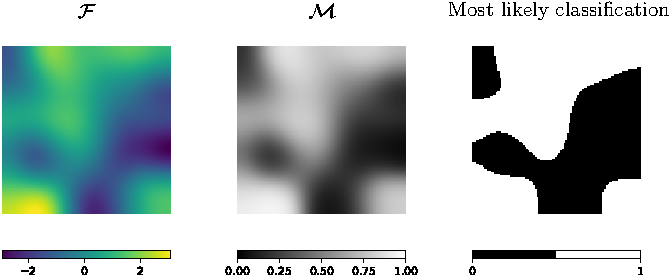
\includegraphics[width=0.9
        \linewidth]{Figures/logistic_gsr.pdf}
    \end{center}
    \caption[Visualisation of binary classification on a 2D lattice]{An example visualisation of binary classification on a $100 \times 100$ grid of pixels ($N_1 = 100, N_2 = 100$). Left: a random smooth graph signal $\Ft$. Middle: the value of the tensor $\Mt$ found by applying the logistic link function of \cref{eq:logistic_link}. Right: the resultant most likely classification given by $\Mt_{\nn} > 0.5$ each pixel, $\nn$.} 
    \label{fig:logistic_gsr}
\end{figure} 
 
Through the application of Bayes' rule, we can derive an equation for the posterior distribution of $\Ft$ given $\Yt$. The Maximum A Posteriori (MAP) estimator for $\Ft$ corresponds to the value that minimizes the negative log-likelihood of this distribution. Thus, we introduce the objective function $\xi(\f) $, which is equal to $ -\log p(\f \, | \, \y)$ up to an additive constant not dependent on $\f$.
 
\begin{equation}
    \xi(\f) = -\s^\top \big(\y \circ \log \muu(\f) + \left(\one  - \y\right) \circ \log \left(\one - \muu(\f) \right)\big) + \frac{\gamma}{2} \f^\top \HH^{-2} \f
\end{equation}

\subsection{Solving with the IRLS algorithm}

Unlike the normal models of the previous sections, no closed-form solution exists to minimise this expression. A standard approach to solving optimisation problems of this form is to use the Iteratively Reweighted Least Squares (IRLS) algorithm. IRLS algorithms have been independently discovered several times and have been studied for over 50 years. Their main use today is found in $L^p$ norm optimisation problems such as sparse recovery (e.g. \cite{Gorodnitsky1997,Daubechies2010}) and maximum likelihood estimation within a generalized linear models \citep{Nelder1972}. 

The IRLS algorithm begins with an initial estimate $\f_0$, which is then iteratively refined to reach the global minimum. Each step is given by the following update formula. 

\begin{equation}
    \label{eq:irls_update}
    \f_{k+1} = \f_{k} - \PP^{-1}(\f_k) \, \g(\f_k)
\end{equation}

where $ \g(\f) \in \R^N$ is the gradient of the optimisation objective $\xi(\f)$ with respect to the vector $\f$, and $\PP(\f) \in \R^{N \times N}$ is the Hessian, which is the matrix of second derivatives such that

\begin{equation*}
    \PP_{nm} = \frac{\partial^2 \xi(\f)}{\partial \f_n \partial \f_m}
\end{equation*}

In our case, the gradient is given by 

\begin{equation}
    \g(\f) = \frac{\partial \xi(\f)}{\partial \f} = \D_\St \big(\muu(\f) - \y\big) + \gamma \HH^{-2} \f
\end{equation}

and the Hessian is given by 

\begin{equation}
    \label{eq:logistic_gsr_P}
    \PP(\f) = \frac{\partial \g(\f)}{\partial \f} =  \D_{\muu}(\f) + \gamma \HH^{-2}
\end{equation}

where $\D_{\muu}(\f)$ is a diagonal matrix with the following definition. 

\begin{equation*}
    \D_{\muu}(\f) = \text{diag}\big(\s \circ \muu(\f) \circ (\one - \muu(\f))\big)
\end{equation*}

A derivation of the expressions for both gradient and the Hessian can be found in \cref{the:gradient_and_hesian}. Note that they are both a function of $\f$. Consider the IRLS update formula given in \cref{eq:irls_update}. Substituting in the values for $\PP$ and $\g$, and using the shorthands

\begin{equation*}
    \PP(\f_k) = \PP_k, \quad \g(\f_k) = \g_k, \quad \muu(\f_k) = \muu_k, \aand \D_{\muu}(\f_k) = \D_{\muu}^k
\end{equation*}

gives

\begin{align*}
    \f_{k+1} &= \f_k - \PP^{-1}_k \, \g_k\\
    &= \f_{k} - \PP^{-1}_k \left(\D_\St \big(\muu_k - \y\big) + \gamma \HH^{-2} \f_k\right) \\
    &= \f_k + \PP^{-1}_k \D_\St \big(\y - \muu_k\big) - \PP^{-1}_k (\gamma \HH^{-2} \f_k) \\
    &= \PP^{-1}_k \D_\St \big(\y - \muu_k \big) + \PP^{-1}_k \left(\PP_k \f_k - \gamma \HH^{-2} \f_k\right) \\
    &= \PP^{-1}_k \D_\St \big(\y - \muu_k \big) + \PP^{-1}_k \D_{\muu}^k\f_k  \\
    &= \PP^{-1}_k \left(\D_\St \big(\y - \muu_k \big) + \D_{\muu}^k\f_k \right) \\
    &= \PP^{-1}_k \tee_k
\end{align*}

where

\begin{equation}
    \tee_k = \D_\St \big(\y - \muu_k\big) + \D_{\muu}^k \f_k
\end{equation}

Hence, each iteration of the IRLS algorithm reduces to solving the linear system $\PP^{-1}_k \tee_k$, for some vector $\tee_k$. 

\subsection{Completing iterations with the CGM}

When it comes to solving the linear system $\PP^{-1}_k \tee_k$, we encounter similar challenges to those discussed in previous chapters. Specifically, the implicit dimensionality of $\PP_k$ can be substantial for tensor-valued graph signals, and the inverse-squared filter matrix $\HH^{-2}$ appearing in the definition of $\PP_k$ [see \cref{eq:logistic_gsr_P}] may suffer from ill-conditioning. Once again, these issues can be overcome by employing the SIM or CGM techniques introduced earlier in \cref{sec:SIM,sec:CGM}.


In this chapter, our focus will be on the CGM for two primary reasons. Firstly, as the dimensionality of tensor-valued binary graph signals increases, it is likely that only a small fraction of nodes will have valid observed data in most practical applications. As demonstrated in \cref{sec:GSR_convergence_implications}, the CGM exhibits superior scaling properties when the input graph signal $\Yt$ is sparsely observed. Secondly, when it comes to sampling from the posterior distribution, certain aspects of the CGM can be reused, as discussed in \cref{sec:GSR_PO}. In this chapter, we also analyse sampling-related questions in \cref{sec:lsamp} and utilise the CGM method. Hence, for the sake of simplicity, it is preferable to use the CGM in both cases instead of mixing methods.

Recall that the CGM seeks to solve a linear system by introducing the symmetric preconditioner $\PSI$, for the purpose of reducing the condition number of the coefficient matrix. In the case of logistic GSR, we can obtain an alternative expression for the update formula with a reduced condition number as follows. 

\begin{equation*}
    \f_k = \PP^{-1}_k \tee_k \quad \Longrightarrow \quad \f_k = \PSI \Q_k^{-1} \PSI^\top \tee_k
\end{equation*}

where, as in previous sections, 

\begin{equation*}
    \PSI = \U \D_\Gt
\end{equation*}

By instead solving the linear system $\Q_k^{-1} (\PSI^\top \tee_k)$ using the conjugate gradient method, and then left-multiplying the result by $\PSI$, we can obtain $\f_{k+1}$ with fewer iterative steps than solving $\PP^{-1} \tee_k$ directly. In this case, $\Q_k$ is given by the following expression. 

\begin{equation}
    \label{eq:Q_LGSR}
    \Q_k = \D_\Gt \U^\top \D_{\muu}^k \U \D_\Gt + \gamma \I_N
\end{equation}

While the condition number, $\kappa$, of $\PP$ is potentially unbounded, $\kappa(\Q)$ is guaranteed to have a maximum value of $(0.25 + \gamma) / \gamma$, as shown formally in \cref{the:L_GSR_Q_conditioning}. 

\begin{theorem}
    \label{the:L_GSR_Q_conditioning}
    
    The condition number of $\Q_k$ is bounded by a maximum value of 
    
    \begin{equation}
        \kappa(\Q_k) \leq \frac{0.25 + \gamma}{\gamma}
    \end{equation}

\end{theorem}

\begin{proof}
    As established in \cref{sec:wfl_derivation}, the worst-case convergence rate is achieved in the limit of a weak filter, where $\D_\Gt = \I_N$. In this case, the condition number of $\Q_k$ is given by 

    \begin{align*}
        \kappa(\Q_k) &= \kappa\left( \U^\top \D_{\muu}^k \U + \gamma \I_N\right) \\[0.1cm]
        &=  \kappa\left( \U^\top \left(\D_{\muu}^k + \gamma \I_N\right) \U  \right) \\[0.1cm]
        &= \kappa\left( \D_{\muu}^k + \gamma \I_N\right)
    \end{align*}

    Since $\D_{\muu}^k = \text{diag}\big(\s \circ \muu_k \circ (\one - \muu_k)\big)$, the maximum possible value along the diagonal of $\D_{\muu}^k$ will be 0.25, occurring when the corresponding element of $\muu_k$ is $1/2$. Furthermore, since $\s$ is a binary vector, the smallest possible value along the diagonal is 0. Therefore, the ratio between the largest and smallest eigenvalues of $ \D_{\muu}^k + \gamma \I_N$ must be less than or equal to $(0.25 + \gamma) / \gamma$. 
\end{proof}



\begin{algorithm}[ht]
    \begin{algorithmic}
    \vspace{0.15cm}
    \Require{Observed binary tensor $\Yt \in \{0, 1\}^{N_1 \times ... \times N_d}$}
    \vspace{0.05cm}
    \Require{Binary sensing tensor $\St \in \{0, 1\}^{N_1 \times ... \times N_d}$}
    \vspace{0.05cm}
    \Require{Cartesian product graph Laplacian $\LL \in \R^{N \times N}$}
    \vspace{0.05cm}
    \Require{Regularisation parameter $\gamma \in \R^+$}
    \vspace{0.05cm}
    \Require{Graph filter function $g(\, \cdot\, \,; \betaa)$}
    \vspace{0.25cm}
    \State{Decompose $\LL$ into $\U \LAM \U^\top$ }
    \vspace{0.15cm}
    \State{Compute $\Gt \in \R^{N_1 \times ... \times N_d}$ as $\Gt_{\nn} = g\big(\lambdaa(\nn); \, \betaa\big)$ }
    \vspace{0.15cm}
    \State{$\D_\Gt \leftarrow \diag{\vecrm{\Gt}}$}
    \vspace{0.15cm}
    \State{$\D_\St \leftarrow \diag{\vecrm{\St}}$}
    \vspace{0.15cm}
    \State{$\PSI \leftarrow \U \D_\Gt$}
    \vspace{0.15cm}
    \State{Initialise $\f \in \R^N$ randomly}
    \vspace{0.15cm}
    \While{$|\Delta \f| > \text{tol}$}
    \vspace{0.15cm}
    \State{$\muu \leftarrow \one / \big(\one + \exp(-\f)\big)$}
    \vspace{0.15cm}
    \State{$\D_{\muu} \leftarrow  \diag{\vecrm{\s \circ \muu \circ (1 - \muu)}}$}
    \vspace{0.15cm}
    \State{$\tee \leftarrow \D_\St \big(\y - \muu\big) + \D_{\muu} \f $}
    \vspace{0.15cm}
    \State{$\Q \leftarrow  \D_\Gt \U^\top \D_{\muu} \U \D_\Gt + \gamma \I_N$}
    \vspace{0.15cm}
    \State{$\f \leftarrow \PSI \Q^{-1} \PSI^\top \tee \quad$ solve with the CGM}
    \vspace{0.15cm}
    \EndWhile
    \vspace{0.15cm}
    \Ensure{$\one / \big(\one + \exp(-\f)\big)$}
    \end{algorithmic}
    \caption{Logistic Graph Signal Reconstruction}
    \label{al:LGSR}
\end{algorithm}

For completeness, we now give the full algorithm for logistic graph signal reconstruction in \cref{al:LGSR}. Note that, by making use of the fast Kronecker product algorithm described in \cref{sec:fast_kron_dd}, the runtime complexity of the CGM step is bounded by 

\begin{equation*}
    O\left(\frac{0.25 + \gamma}{\gamma} N \sum_{i=1}^d N_i \right)
\end{equation*}

The run time complexity of the overall algorithm of course depends on the convergence rate of the IRLS iterations. This is known to be super-linear, and approximately quadratic when a sufficiently accurate starting value is used \citep{Burden2010}. Whilst an in-depth theoretical exploration of the IRLS algorithm for this particular application is beyond the scope of this chapter, in practice, the IRLS algorithm converges very quickly, usually taking on the order of 10 steps to achieve negligible error.


\section{Logistic Graph Signal Regression} 

 
\label{sec:logistic_regression}

\subsection{L-KGR}

\label{sec:lkgr}

\section{L-RNC}

\label{sec:lrnc}

\subsection{L-KG-RNC}

\label{sec:lkgrnc}

\section{Multiclass Methods}

\label{sec:multiclass}

Up to this point in the chapter, our focus has been on binary-valued graph signals, which can be used to represent two-class classification tasks over a multiway network. However, in many practical applications, the task may involve classifying each node into one of multiple distinct groups. Therefore, the objective of this section is to extend and generalise the methods we have developed thus far to encompass multiclass classification problems.

Let us first consider the task of multiclass graph signal reconstruction. Here, the goal is to classify each node, $\nn$, in a $d$-dimensional Cartesian product graph into one of $C>2$ distinct groups. To do this, we have access to the graph Laplacian $\LL \in \R^{N \times N}$, and the true class label at a subset of nodes, $\mathcal{S}$. This partially observed graph signal can be represented as an order-($d + 1$) tensor, where the last dimension contains a ``one-hot" encoding of the class label. As such, the input data can be summarised as follows. 

\begin{equation*}
    \text{input data} = \Big\{\; \Yt \in \{0, 1\}^{N_1 \times ... \times N_d \times C}, \;\; \St \in \{0, 1\}^{N_1 \times ... \times N_d} , \;\; \LL \in \R^{N \times N} \; \Big\}
\end{equation*}

As in previous sections, the tensor $\St$, of shape $(N_1 \times ... \times N_d$), indicates which nodes in the product graph have been successfully observed by holding a one in the corresponding entry, and zeros elsewhere. Note that the observed graph signal, $\Yt$, has an additional dummy dimension of length $C$ to represent the class label. Where no observation was made, the corresponding values of $\Yt_{\nn, :}$ can all be safely set to zero. 

We describe the probability that node $\nn$ has class $c$ with another tensor, $\Mt$, which, like $\Yt$, has shape $(N_1 \times ... \times N_d \times C)$. In particular, 

\begin{equation*}
    p(\text{node} \; \nn \; \text{is of class} \; c) = \Mt_{\nn, c}
\end{equation*}

Given this, the probability of observing a signal $\Yt$ for a given mean $\Mt$ is

\begin{equation}
    p(\Yt \, | \, \Mt) = \prod_{c, \nn \in \mathcal{S}} \Mt_{\nn, c}^{\Yt_{\nn, c}}
\end{equation}

As such, the log-likelihood of observing a signal $\Yt$ is given by 

\begin{equation}
   \log p(\Yt \, | \, \Mt) = (\s \otimes \one_C)^\top \big(\y \circ \log \muu \big)
\end{equation}

where, as before, $\s = \vecrm{\St}, \; \y = \vecrm{\Yt}$ and $\muu = \vecrm{\Mt}$. Furthermore, to enforce the restriction that all probabilities must sum to one, we can generate $\Mt$ by applying a softmax function to a tensor $\Ft$. 

\begin{equation}
    \label{eq:softmax}
    \Mt_{\nn, c} = \frac{\exp(\Ft_{\nn, c})}{ \raisebox{-0.1cm} { $\sum_{c'=1}^C \exp(\Ft_{\nn, c'})$ }}  \quad \Longleftrightarrow \quad \muu(\f) = \frac{\exp(\f)}{ \big((\I_N \otimes \one_C) \exp(\f)\big) \otimes \one_C}
\end{equation}

Here, $\Ft$ is a real-valued tensor signal which, like $\Mt$ and $\Yt$, has shape $(N_1 \times ... \times N_d \times C)$. A graphical representation of the relation between $\Ft$, $\Mt$ and the most likely classification is shown in \cref{fig:logistic_gsr_multiclass}. The goal, then, of multiclass logistic graph signal reconstruction is to find the most likely value for the tensor $\Ft$, which allows us to make a prediction for the probability of each class by applying \cref{eq:softmax}.  

\begin{figure}[t]  
    \begin{center}
        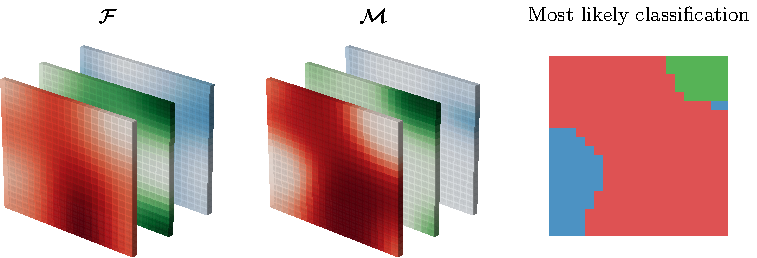
\includegraphics[width=\linewidth]{Figures/multiclass.pdf}
    \end{center}
   \caption[Visualisation of multiclass classification on a 2D lattice]{An example visualisation of multiclass classification on a $20 \times 20$ grid of pixels ($N_1 = 20, N_2 = 20, C=3$). Left: a random smooth tensor signal $\Ft$ split across three channels. Middle: the value of the tensor $\Mt$ found by applying the softmax function of \cref{eq:softmax} in the class dimension. Right: the resultant most likely classification given by the maximum probability class label for each pixel. } 
    \label{fig:logistic_gsr_multiclass}
\end{figure} 


Assuming no particular relational structure between the $C$ classes, we can encode the assumption that class probabilities should vary smoothly over the graph by assigning the following prior to $\Ft$. 

\begin{equation}
    \f \sim \Norm{\zero}{\gamma^{-1} \HH^2 \otimes \I_C}
\end{equation}

By applying Bayes' rule, we can therefore derive an expression $\xi(\f)$, representing the posterior log-likelihood of an underlying signal $\f$ given an observed signal $\y$. 

\begin{equation*}
    \xi(\f) = - (\s \otimes \one_C)^\top \big(\y \circ \log \muu(\f) \big) + \frac{\gamma}{2} \f^\top \left(\HH^{-2} \otimes \I_C\right) \f
\end{equation*}

Once again, we can solve for the minimising value of $\f$ using the IRLS algorithm. In this case, the gradient and Hessian are respectively given by 

\begin{equation}
    \g(\f) = \big(\D_\St \otimes \I_C\big) \big(\muu(\f) - \y\big) + \gamma \left(\HH^{-2} \otimes \I_C\right) \f
\end{equation}

and

\begin{equation}
    \PP(\f) = \RR_{\muu}(\f) + \gamma \HH^{-2} \otimes \I_C
\end{equation}

where, unlike the binary case where the Hessian was the sum of a diagonal matrix $\D_{\muu}(\f)$ and $\gamma \HH^{-2}$, the matrix $\RR_{\muu}(\f)$ is no longer diagonal. First, let us define the matrix $\M$ to be the tensor $\Mt$ reshaped in row major order to have dimensions $(N \times C)$. Then, the $\RR_{\muu}(\f)$ is given by 

\begin{equation}
    \RR_{\muu}(\f) =  \big(\D_\St \otimes \I_C\big) \left(\Diag{\muu(\f)} - \sum_{n=1}^N \mathbf{\Delta}_{n} \otimes \M_n (\f) \M_n^\top(\f) \right)
\end{equation}

where $\M_n$ is the $n$-th row of $\M$ and $\mathbf{\Delta}_{n}$ is a matrix of zeros, with a single one at element $(n, n)$. Given the definition of the Kronecker product, we can see that $\RR_{\muu}(\f)$ is a block-diagonal matrix with the following structure. 

\begin{equation*}
    \RR_{\muu}(\f) = \begin{bmatrix}
        \B_1 & & & \\
        & \B_2 & & \\
        & & \ddots & \\
        & & & \B_N
    \end{bmatrix}, \quad \text{where} \quad \B_n = \s_n \Big(\diag{\M_n} - \M_n \M_n^\top\Big)
\end{equation*}

where $\OO_C$ is a $(C \times C)$ matrix of zeros. Despite no longer being diagonal, we can still leverage the block structure of this matrix to multiply $\RR_{\muu}(\f)$ onto an arbitrary vector, $\ve$, efficiently. This can be achieve as follows. 


\begin{equation}
    \label{eq:R_mu_eff}
    \RR_{\muu}(\f) \ve = (\s \otimes \one_C) \circ  \muu(\f) \circ \ve - \Big(\big((\D_\St \otimes \one_C) (\muu(\f) \circ \ve) \big) \otimes \one_C \Big) \circ \muu(\f)
\end{equation}

While a naive implementation of the product $\RR_{\muu}(\f) \ve$ would have memory time and memory complexity $O\left(C^2N^2\right)$, by following the formula given in \cref{eq:R_mu_eff}, it can instead be achieved with $O(NC)$ for both, as it would for a diagonal operator of size $(NC \times NC)$. 

Now consider the IRLS update formula. As before, we will use the following shorthands. 

\begin{equation*}
    \PP(\f_k) = \PP_k, \quad \g(\f_k) = \g_k, \quad \muu(\f_k) = \muu_k, \aand \RR_{\muu}(\f_k) = \RR_{\muu}^k
\end{equation*}

Applying the update formula gives

\begin{align*}
    \f_{k+1} &= \f_k - \PP^{-1}_k \, \g_k\\
    &= \f_{k} - \PP^{-1}_k \Big(\big(\D_\St \otimes \I_C\big) \big(\muu_k - \y\big) + \gamma \left(\HH^{-2} \otimes \I_C\right) \f_k\Big) \\
    &= \f_k + \PP^{-1}_k \big(\D_\St \otimes \I_C\big) \big(\y - \muu_k\big) - \PP^{-1}_k \Big(\gamma \left(\HH^{-2} \otimes \I_C\right) \f_k\Big) \\
    &= \PP^{-1}_k \big(\D_\St \otimes \I_C\big) \big(\y - \muu_k \big) + \PP^{-1}_k \Big(\PP_k \f_k - \gamma \left(\HH^{-2} \otimes \I_C\right) \f_k\Big) \\
    &= \PP^{-1}_k \big(\D_\St \otimes \I_C\big) \big(\y - \muu_k \big) + \PP^{-1}_k \RR_{\muu}^k\f_k  \\
    &= \PP^{-1}_k \left(\big(\D_\St \otimes \I_C\big)\big(\y - \muu_k \big) + \RR_{\muu}^k\f_k \right) \\
    &= \PP^{-1}_k \tee_k
\end{align*}

where 

\begin{equation*}
    \tee_k = \big(\D_\St \otimes \I_C\big)\big(\y - \muu_k \big) + \RR_{\muu}^k\f_k
\end{equation*}

As before, we can solve the linear system $\PP^{-1}_k \tee_k$ by introducing a symmetric preconditioner $\PSI$. The only modification is that it must be of dimension of $(NC \times NC)$, rather than $(N \times N)$. This can be achieved as follows. 

\begin{equation*}
    \PSI = \U \D_\Gt \otimes \I_C 
\end{equation*}

Using this, we can transform the linear system into 

\begin{equation*}
    \f_k = \PP^{-1}_k \tee_k \quad \Longrightarrow \quad \f_k = \PSI \Q_k^{-1} \PSI^\top \tee_k
\end{equation*}

where 

\begin{equation}
    \label{eq:Q_LGSR_mc}
    \Q_k = \big(\U \D_\Gt \otimes \I_C\big)^\top  \RR_{\muu}^k \big(\U \D_\Gt \otimes \I_C\big) + \gamma \I_{NC}
\end{equation}

While the condition number, $\kappa$, of $\PP$ is potentially unbounded, $\kappa(\Q)$ is guaranteed to have a maximum value of $(0.5 + \gamma) / \gamma$, as shown formally in \cref{the:L_GSR_mc_Q_conditioning}. 

\begin{theorem}
    \label{the:L_GSR_mc_Q_conditioning}
    
    The condition number of $\Q_k$ is bounded by a maximum value of 
    
    \begin{equation}
        \kappa(\Q_k) \leq \frac{0.5 + \gamma}{\gamma}
    \end{equation}

\end{theorem}

\begin{proof}
    As established in \cref{sec:wfl_derivation}, the worst-case convergence rate is achieved in the limit of a weak filter, where $\D_\Gt = \I_N$. In this case, the condition number of $\Q_k$ is given by 

    \begin{align*}
        \kappa(\Q_k) &= \kappa\left( (\I_C \otimes \U)^\top \RR_{\muu}^k (\I_C \otimes \U) + \gamma \I_{NC}\right) \\[0.1cm]
        &=  \kappa\left( (\I_C \otimes \U)^\top \left(\RR_{\muu}^k + \gamma \I_N\right) (\I_C \otimes \U)  \right) \\[0.1cm]
        &= \kappa\left( \RR_{\muu}^k + \gamma \I_N\right)
    \end{align*}

    Since $\RR_{\muu}^k$ is block-diagonal, its eigenvalues are equal to the union of the eigenvalues of each individual block. Consider the characteristic equation for the eigenvalues of block $\B_n$, given by 

    \begin{equation*}
        \B_n = \s_n \Big(\diag{\M_n} - \M_n \M_n^\top\Big)
    \end{equation*}
    
    For the case where $\s_n \neq 0$, the characteristic equation is

    \begin{equation*}
        f(\lambda) = 1 - \sum_{c=1}^C \frac{(\M_n)_c^2}{(\M_n)_c - \lambda}
    \end{equation*}

    Consider the value of $f(0)$. 
    
    \begin{align*}
        f(0) &= 1 - \sum_{c=1}^C \frac{(\M_n)_c^2}{(\M_n)_c} \\
        &= 1 - \sum_{c=1}^C (\M_n)_c \\
        &= 0
    \end{align*}

    where the final line follows from the fact that probabilities must sum to one. Therefore, every block will have at least one zero eigenvalue. Now consider the limit of $f(\lambda)$ as $\lambda \rightarrow \infty$. Clearly this is one. Furthermore, $f(\lambda)$ has $C$ asymptotes, occurring at $\lambda = (\M_n)_c$. Let us assume without loss of generality that $(\M_n)_c$ are arranged in ascending order. Taken together, this implies that the roots of $f(\lambda)$, denoted in ascending order as $[\lambda_1, \lambda_2, ..., \lambda_C]$ are restricted as follows:

    \begin{equation*}
        \lambda_1 = 0, \quad \lambda_2 < \frac{ (\M_n)_1 +(\M_n)_2}{2}, \quad \quad ...  \quad \lambda_C < \frac{(\M_n)_{C-1} + (\M_C)_2}{2}
    \end{equation*}

    Since the largest eigenvalue must be less than the average of the two largest values of $(\M_n)_c$, we can see that the largest possible eigenvalue of $\RR_{\muu}^k$ is 0.5. As established, the smallest possible eigenvalue is zero. Therefore $\kappa\left( \RR_{\muu}^k + \gamma \I_N\right) \leq (0.5 + \gamma) / \gamma$. 

\end{proof}

For completeness, we now give the full algorithm for logistic graph signal reconstruction in \cref{al:LGSR}. Note that, by making use of the fast Kronecker product algorithm described in \cref{sec:fast_kron_dd}, the runtime complexity of the CGM step is bounded by 

\begin{equation*}
    O\left(\frac{0.5 + \gamma}{\gamma} NC \Big(C + \sum_{i=1}^d N_i \Big)\right)
\end{equation*}

\begin{algorithm}[ht]
    \begin{algorithmic}
    \vspace{0.15cm}
    \Require{Observed binary tensor $\Yt \in \{0, 1\}^{N_1 \times ... \times N_d \times C}$}
    \vspace{0.05cm}
    \Require{Binary sensing tensor $\St \in \{0, 1\}^{N_1 \times ... \times N_d}$}
    \vspace{0.05cm}
    \Require{Cartesian product graph Laplacian $\LL \in \R^{N \times N}$}
    \vspace{0.05cm}
    \Require{Regularisation parameter $\gamma \in \R^+$}
    \vspace{0.05cm}
    \Require{Graph filter function $g(\, \cdot\, \,; \betaa)$}
    \vspace{0.25cm}
    \State{Decompose $\LL$ into $\U \LAM \U^\top$ }
    \vspace{0.15cm}
    \State{Compute $\Gt \in \R^{N_1 \times ... \times N_d}$ as $\Gt_{\nn} = g\big(\lambdaa(\nn); \, \betaa\big)$ }
    \vspace{0.15cm}
    \State{$\D_\Gt \leftarrow \diag{\vecrm{\Gt}}$}
    \vspace{0.15cm}
    \State{$\D_\St \leftarrow \diag{\vecrm{\St}}$}
    \vspace{0.15cm}
    \State{$\PSI \leftarrow \U \D_\Gt \otimes \I_C$}
    \vspace{0.15cm}
    \State{Initialise $\f \in \R^{NC}$ randomly}
    \vspace{0.15cm}
    \While{$|\Delta \f| > \text{tol}$}
    \vspace{0.15cm}
    \State{$\muu \leftarrow \exp(\f) / \big((\I_N \otimes \one_C) \exp(\f)\big) \otimes \one_C$}
    \vspace{0.15cm}
    \State{$\M \leftarrow \text{reshape}\big(\muu, (N, C)\big)$}
    \vspace{0.15cm}
    \State{$\RR_{\muu} \leftarrow  \big(\D_\St \otimes \I_C\big) \left(\Diag{\muu} - \sum_{n=1}^N \mathbf{\Delta}_{n} \otimes \M_n \M_n^\top \right)$}
    \vspace{0.15cm}
    \State{$\tee \leftarrow \big(\D_\St \otimes \I_C\big)\big(\y - \muu \big) + \RR_{\muu}\f$}
    \vspace{0.15cm}
    \State{$\Q \leftarrow  \big(\U \D_\Gt \otimes \I_C\big)^\top  \RR_{\muu} \big(\U \D_\Gt \otimes \I_C\big) + \gamma \I_{NC}$}
    \vspace{0.15cm}
    \State{$\f \leftarrow \PSI \Q^{-1} \PSI^\top \tee \quad$ solve with the CGM}
    \vspace{0.15cm}
    \EndWhile
    \vspace{0.15cm}
    \Ensure{$\f$}
    \end{algorithmic}
    \caption{Multiclass Logistic Graph Signal Reconstruction}
    \label{al:LGSR_mc}
\end{algorithm}

\section{Approximate Sampling via the Laplace Approximation}

\label{sec:lsamp}

